\section{Description séquentielle des modules}
    \label{sec:modules}
    
Les diagrammes de séquences présentés dans cette partie ont pour objectif d'illustrer le fonctionnement des trois principales fonctionnalités de Glasir : le Filtre, l'Optimiseur et l'Editeur de fonction. Chaque diagramme commence par l'ouverture d'un ADTree dans Glasir, représenté par le bloc \og Start \fg{}.

	\subsection{Filtre}

	    \begin{figure}[H]
	        \centering
	        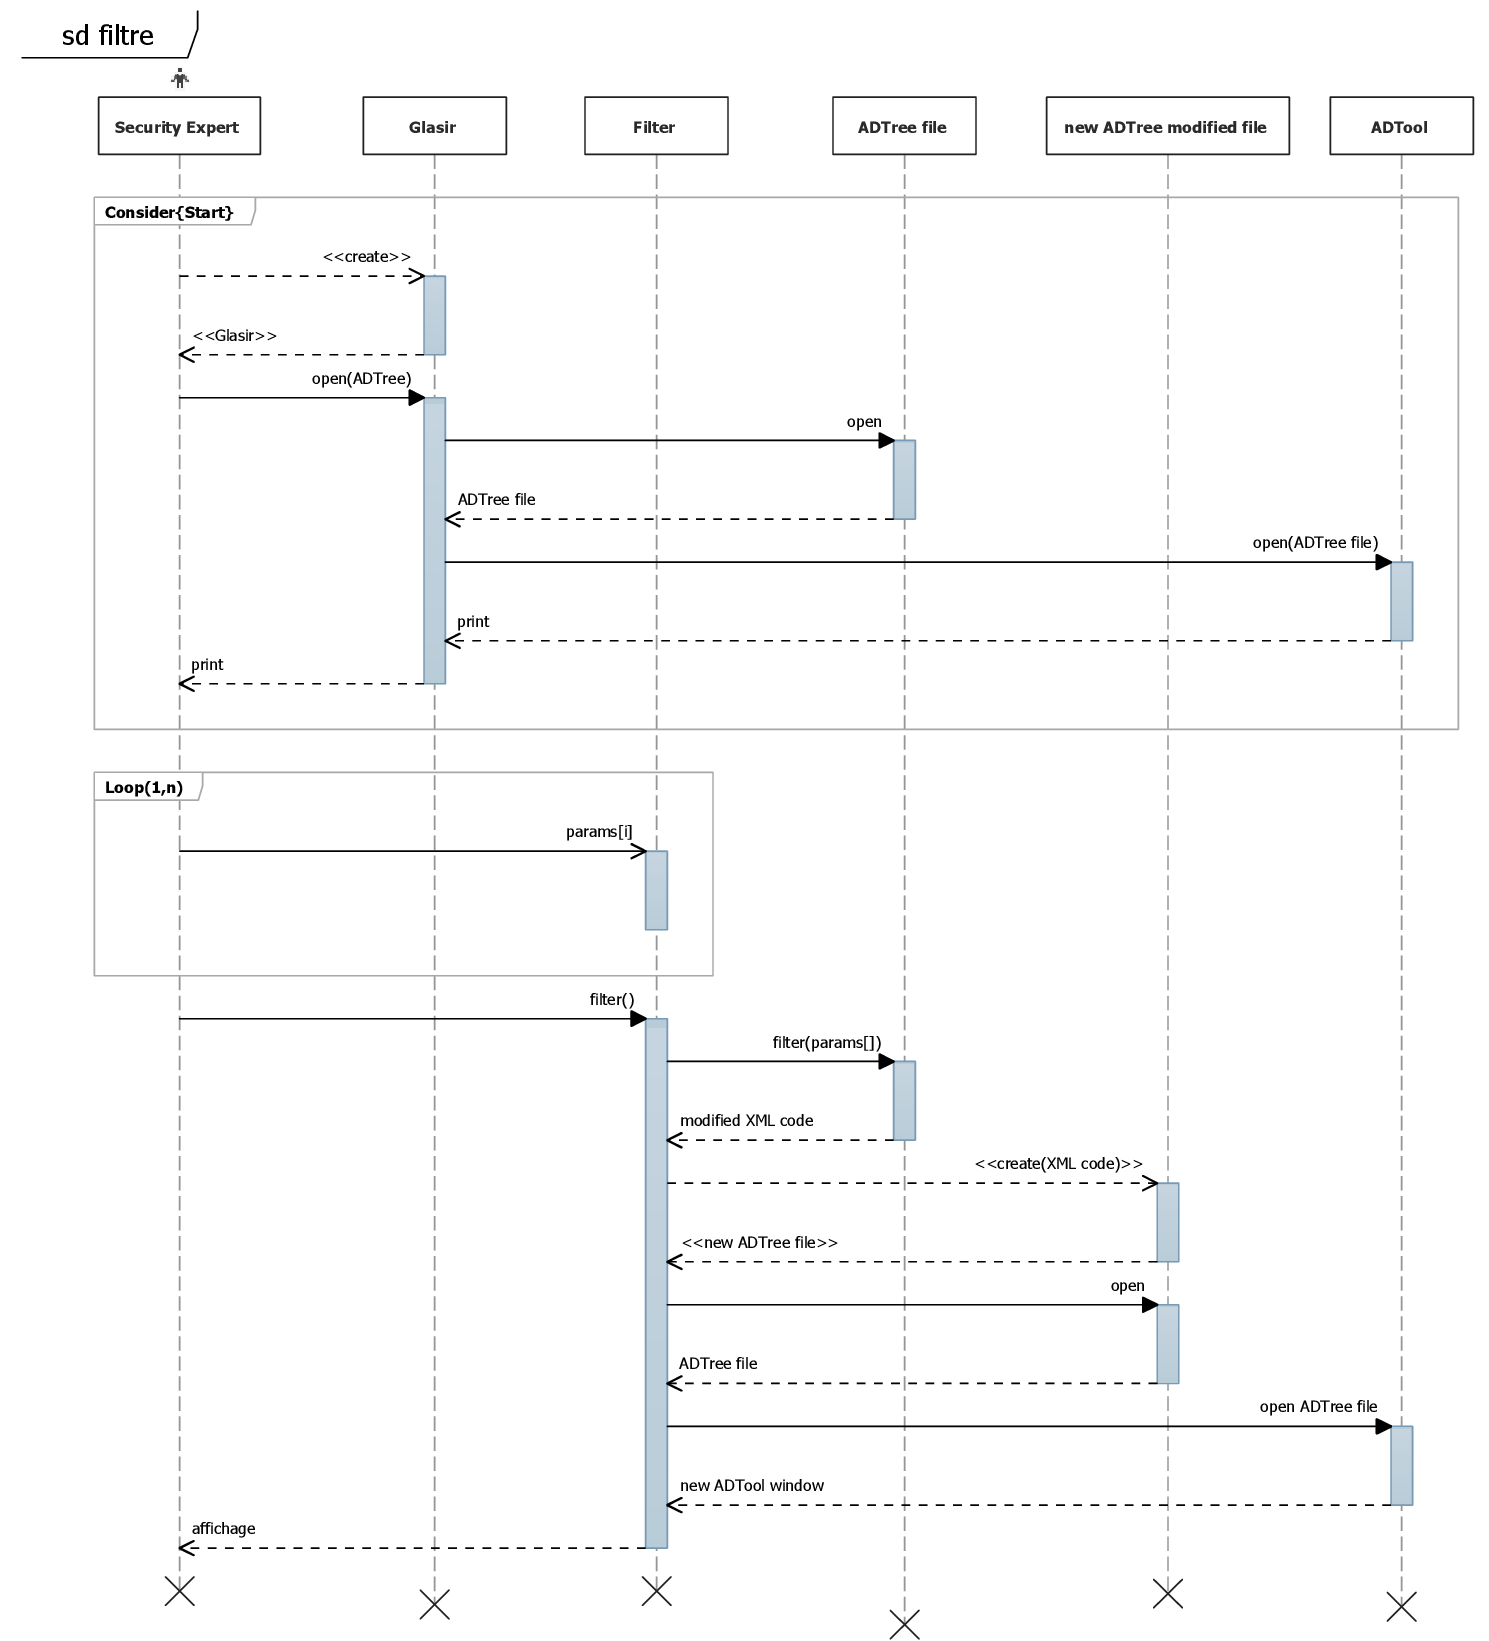
\includegraphics[height=1\textwidth]{figure/Filter.png}
	        \caption{Diagramme de séquence du module Filtre.}
	        \label{fig:filter}
	    \end{figure}

Pour réaliser le filtrage d'un ADTree, l'expert en sécurité va définir des intervalles de filtrage sur les valuations de l'ADTree, et les passer en paramètre au Filtre. Ce dernier va alors analyser le code XML de l'ADTree-cible, afin de produire le code XML de l'ADTree-résultat. Ce code va alors permettre de créer un nouveau fichier contenant l'ADTree-résultat, qui sera alors affiché dans une nouvelle instance d'ADTool.

	\subsection{Optimiseur}

	    \begin{figure}[H]
	        \centering
	        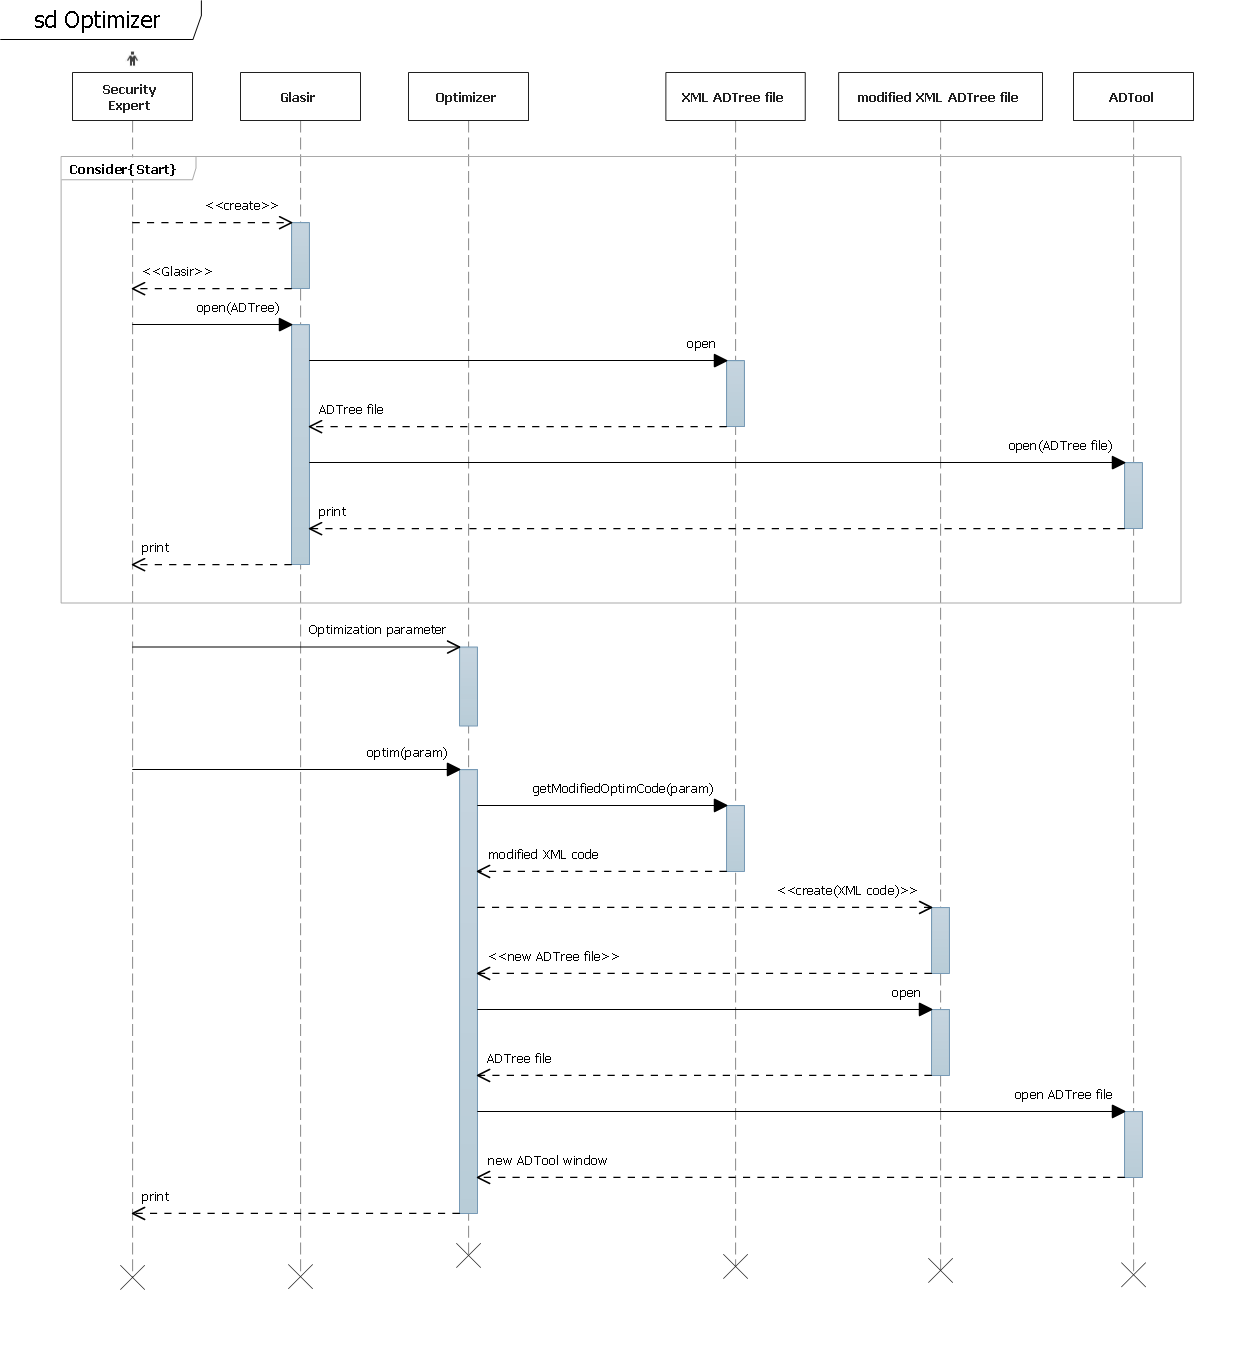
\includegraphics[height=1\textwidth]{figure/Optim.png}
	        \caption{Diagramme de séquence du module Optimiseur.}
	        \label{fig:optim}
	    \end{figure}

Pour réaliser l'optimisation d'un ADTree, l'expert en sécurité va sélectionner la valuation de l'ADTree selon laquelle il souhaite l'optimiser. Il va ensuite lancer l'optimiseur, qui va analyser le code XML de l'ADTree-cible afin de produire le code XML de l'ADTree optimisé. Ce code va alors permettre de créer un nouveau fichier contenant l'ADTree optimisé, qui sera alors affiché dans une nouvelle instance d'ADTool.

	\subsection{Éditeur de fonctions}

	    \begin{figure}[H]
	        \centering
	        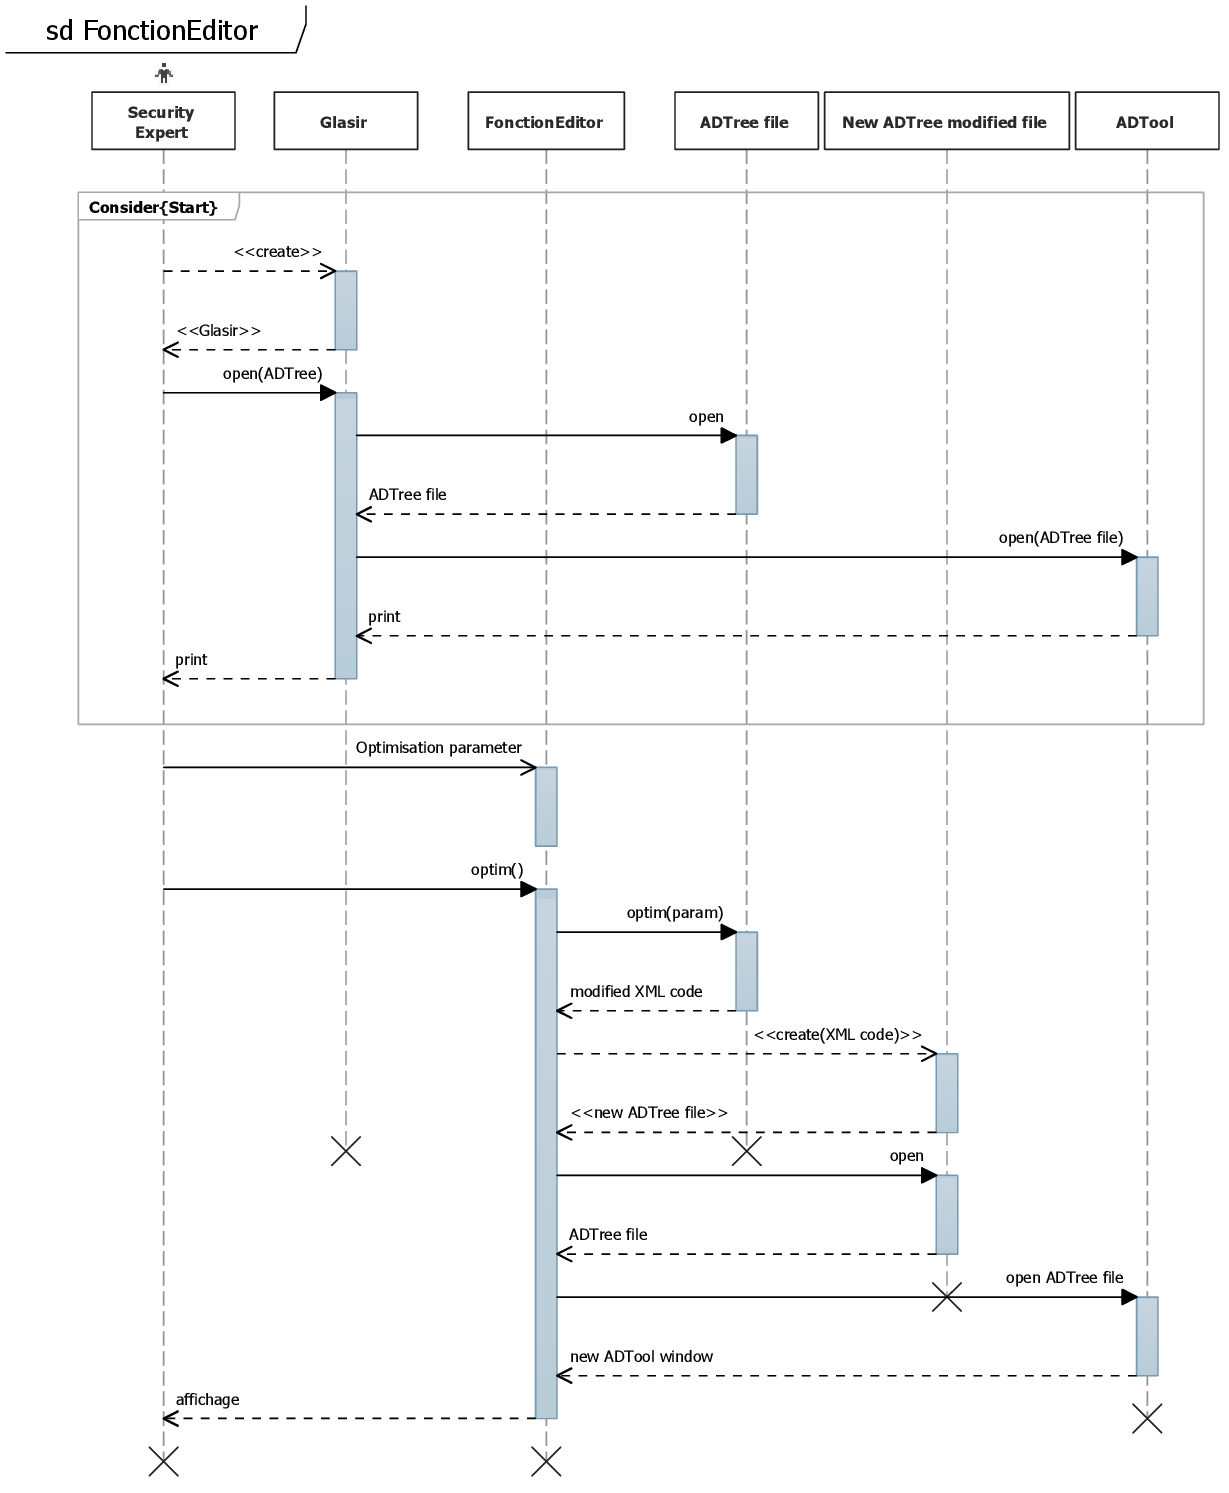
\includegraphics[height=1\textwidth]{figure/FunctionEditor.png}
	        \caption{Diagramme de séquence du module Éditeur de fonctions.}
	        \label{fig:function}
	    \end{figure}

Pour ajouter un nouveau paramètre de valuation à l'ADTree, l'expert en sécurité va commencer par écrire la fonction de calcul de ce paramètre en fonction des valuations déjà présentes. Il va ensuite lancer l'éditeur de fonctions, qui va analyser le code XML de l'ADTree-cible afin de génerer le code XML de l'ADTree avec la valuation supplémentaire. Il va alors créer un nouveau fichier XML dans lequel va être inscrit ce code. Ce code va permettre de créer un nouveau fichier contenant l'ADTree avec la nouvelle valuation, et l'ADTree sera enfin affiché dans une nouvelle instance d'ADTool.